% include the figures path relative to the master file
% \graphicspath{ {./content/method/figures/visual_cues/}{./content/method/figures/}}
\graphicspath{ {./content/method/figures/}}

\section{Materials and Methods}

 This section offers a general description of the methodology proposed for OCT volume classification, whereas further details of some elements involved in the methodology are found as subsections.
  
  The proposed method, as well as, its experimental set-up are outlined in Fig.\,\ref{fig:ML-scheme}.
  The methodology is formulated as a standard classification procedure.
  The available dataset with its acompaining \textcolor{red}{GT} are divided into training $(S1,l1)$ and testing $(S2,l2)$. 
  The final goal is to represent $S1$ and $S2$ in the feature space $F$ by supplying $(sxF,l1)$ as a training to a classifier, using the trained classifier to estimate $l2$ from $S2xF$ and comparing the estimation with the \textcolor{red}{GT}.
   To do so, the images forming the OCT volumes are preprocessed using non-local means (NL-means) algorithm \cite{buades2005non}. This algorithm preserve important details and textures of the original image, while reducing the noise.
   The mapping stage is used to determine a discrete set of elements (or structures) $Z$  which is used for representing the volume $s  in S$.
   The feature detection stage correspond to measurements done in $G(Z)$ used for representing $s$ in terms of $ZxG$. 
   This mapping and feature detection steps can be found as a single-steps in the literature.
   The feature extraction procedure combines the elements in $Z$ and its measurements $G(Z)$ to create the final feature space $F$ and project $s$ on it.
   
   The design choices are all illustrated in Fig.\,\ref{fig:ML-scheme} and discussed further in this section. The work here presented does not discuss in detail neither the mapping, nor the adopted classifier, further than this lines.
   As a possible mappings, for representing the volumes, 2D image slices of the volume and \color{red}{7x7x7}\color{black} sliding volumes, have been considered. 
   As a classifier, a \color{red}{Random Forest}\color{black} using 100 trees, has been considered.
   
\begin{figure}[h]
\centering{
  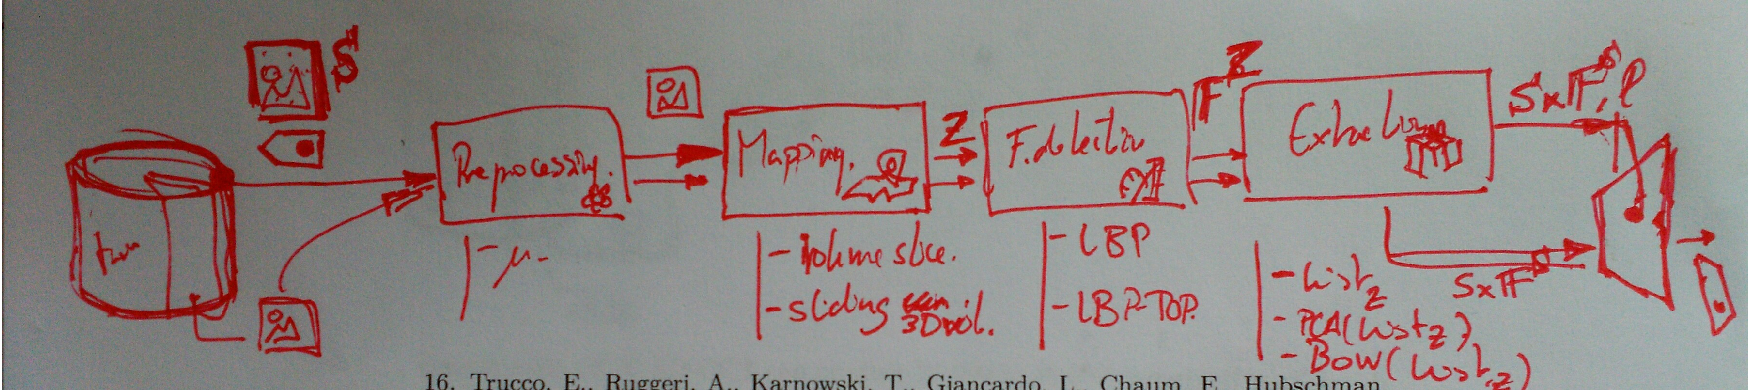
\includegraphics[width=1\textwidth]{mm.pdf}}
  \caption{Machine learning classification basic scheme}
  \label{fig:ML-scheme}
\end{figure}

\subsection{Data}
\color{red}{
\begin{itemize}
  \item cross-validation
  \item our dataset
  \item DUC dataset
\end{itemize}}\color{black}

For evaluation purposes, the results have been cross-validated, by splitting the data in training and testing using a \color{red}{loo}\color{black} strategy. In this manner for each round a pair \color{red}{dce,normal} has been selected to be used as the round test set, while the rest of the dataset has been used as a training. \color{red}{Doing the cross validation in this manner, has the limitation that despite the fact that the results are robust due to the cross validation, no results variance can be reported. However, and despite this limitation, LOO has been choose due to the reduced amount of OCT volumes available.}\color{black}

\color{red}{The dataset blablablabal...}\color{black}
\color{red}{The duc dataset blabla bla...}\color{black}

\subsection{Image pre-processing}
The pre-processing stage in the proposed methodology applies an image denoising method to reduce the speckle noise in OCT images. Since image details and texture of the original image are needed by the following stages in the method, non-local means (NL-means) algorithm \cite{buades2005non} is used. NL-means algorithm has the advantage to use all the possible self-predictions that the image can provide \cite{buades2005non} rather than local or frequency filters such as Gaussian, anisotropic or Wiener filters. \color{red}{Figure .. shows an OCT slice before and after denoising}\color{black}


\subsection{Features extraction}
Need to write something here !!!


\subsubsection{Low-level features} are extracted considering the whole volume using LBP and 3D-LBP descriptors. 
LBP is a discriminative rotation invariant feature descriptor proposed by Ojala et al. \cite{ojala2002multiresolution}. 
LBP descriptor encodes the intensity differences of a central pixel ($g_c$) with its neighboring pixels ($g_{p}$), within in a defined neighborhood of radius $R$. The differences are encoded in terms of binary patterns as in~Eq. \ref{Eq:LBP}: 

\begin{equation} \label{Eq:LBP}
LBP_{P,R} = \sum_{p=0}^{P-1}s(g_{p} - g_{c})2^{p},
\end{equation}
where $s(a) = 1$ if $a \geq 0$, and $s(a)=0$ otherwise. $P$ is the number of sampling points in the circle of radius $R$.

The binary patterns are calculated for each pixel in the given image and their histogram defines the final descriptor.
The LBP histograms are computed for each slice of the volume and are concatenated into a single histogram.


%In this research we consider rotation invariant features with uniform patterns. The uniform patterns are defined by the unifromity measure ($U$) of 2. Uniformity measure corresponds to the number of spatial transitions in the LBP pattern \cite{ojala2002multiresolution}. For instance patterns $00000000_{2}$ and $11111111_{2}$ have the U value of 0 while patterns like $01111111_{2}$ and $00000011_{2}$ have two transitions of 0/1 in their pattern, therfore they are considered as uniform patterns (see Eq. \ref{Eq:LBPru}). 
%\begin{equation}\label{Eq:LBPru}
%  LBP_{P,R}^{riu2} = 
%  \begin{cases}
%     \sum_{p=0}^{P-1}s(g_{p} - g_{c}) & \text{ if } U(LBP_{P,R}) \le 2\\
%       P+1 & \text{otherwise,}
%       \end{cases}
%    \end{equation}


The LBP features are extracted from each B-slice of the volume and their histograms are concatenated to build the first low-level descriptor. The second low-level descriptor is defined in a similar manner as the first one. However principal component analysis (PCA) is applied to the concatenated histograms in order to reduce the dimensions. The first and second low-level descriptors are obtained using the 2D LBP descriptor. However the third low-level feature is obtained using 3D-LBP (LBP-TOP). Zhao et al. \cite{zhao2007dynamic} proposed Local Binary Pattern histogram from Three Orthogonal Planes (LBP-TOP) as a dynamic texture descriptor. This descriptor is an extension to normal LBP while it considers texture descriptors along the temporal domain. LBP-TOP considers the LBP pattern in three orthogonal planes (see Fig. \ref{fig:LBPTOP-framework}), XY, XT and YT. The obtained LBP patterns from the three planes are concatenated to form the final descriptor. 

\begin{figure}
\centering{
  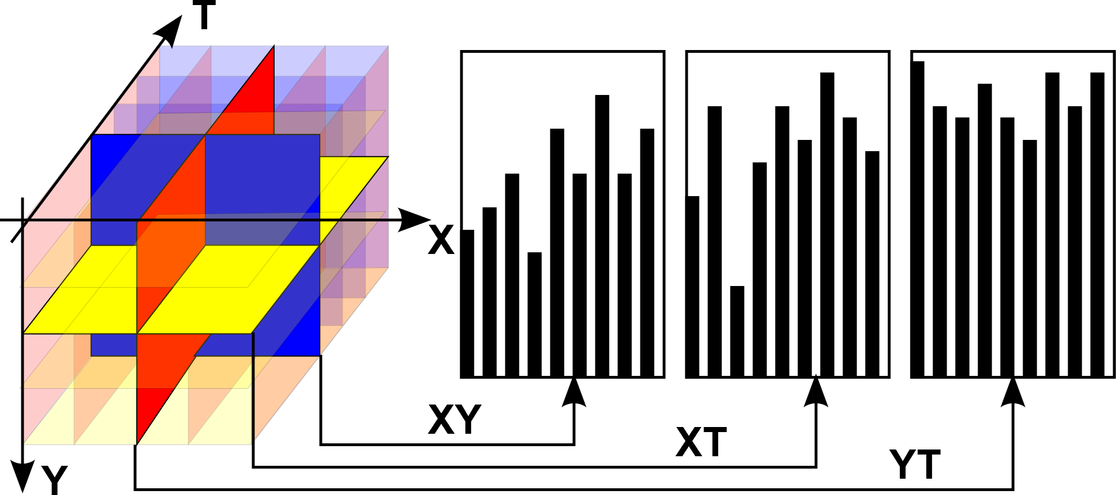
\includegraphics[width=0.40\textwidth]{LBPTOP_fig}}
\caption{LBP-TOP framework, the image is taken from \cite{JiangEtAl13}}
\label{fig:LBPTOP-framework}
\end{figure}



\subsubsection{High-level features} - are extracted using bag of features (BoF) approach which is illustrated in Fig. \ref{fig:BoF-framework}. After de-noising the images by non-local-mean approach, a patch detection step is carried out by identifying informative regions of the data. These patches can either be sampled densely or sparsely. The dense sampling extracts more information regarding the object appearance. However, it might retain redundant features. In the contrary sparse sampling is based on detecting salient key points from the most informative regions of the volume. Our proposed BoF approach is based on the first strategy. In this stage 2D-LBP (7$\times$7) and 3D-LBP-TOP patches (7$\times$7$\times$7) are extracted for each patient. Defining $N$ as the number of selected patches for each volume and $d$ as the number of feature dimensions, then each volume is characterized by a $N \times d$ feature matrix (see Fig. \ref{fig:BoF-framework}, ``feature extraction''). The next step in bag of features consists of building the dictionary of ``visual-words''. All the feature matrices of the training set are concatenated together and k-means clustering method (see Fig.\ref{fig:BoF-framework}, ``clustering'') is used to define the ``visual-words''. K-means is an iterative algorithm which finds k centroids by alternating assignment and update steps. The assignment steps is based on $L_{2}$ norm (Euclidean) distance. Different initialization methods can be used in order to assign the initial k clusters \cite {celebi2013comparative}, here the initial k clusters are selected based on greedy k-means++ method \cite{arthur2007k}. \textbf{Depending on the framework and application, different choices of the number of ``visual-words'' (number of $k$ clusters) can be made. In our framework, the number of clusters are varying in the range of [2 4 8 16 32 64 100]. SHOULD CHNAGE} Finally, the probability distribution (e.g., histogram) of the ``visual-words'' of each feature matrix is computed (feature quantization) and is used to feed the classifier to be trained. In the prediction stage, the histogram of the feature matrix corresponding to the new volume is computed using the previously learned dictionary and, finally, it is classified by the previously trained classifier.\\


% \tikzstyle{block} = [rectangle, draw, fill=gray!20, text = black,
    text width=6em, text centered, rounded corners, minimum height=4em , minimum width = 6em]
    % \tikzstyle{line} = [draw, -latex']
  \tikzstyle{myarrow}=[->, thick]
    \tikzstyle{line}=[-, thick]
    \tikzstyle{block2} = [rectangle, draw, fill=white!20,
    text width=6em, text centered, rounded corners, minimum height=4em, minimum width = 6em]
    \tikzstyle{block3} = [rectangle, draw, fill=gray!20, text = black,
    text width=7em, text centered, rounded corners, minimum height=4em , minimum width = 7em]
\def\blockdist{1}
\def\edgedist{1.5}
  %%%% The Framework Sparse Coding 

\begin{figure}
 \begin{center}
   \begin{tikzpicture}[node distance = 1cm,scale=0.6, every node/.style={scale=0.6}]
%(FEx.east|- FEx.south)
    \node [block2] (input) {Training image};
    %\node [block, right of = input, node distance = 2.8cm](Seg){Segmentation}; 
    \node [block, right of=input,node distance = 2.8cm](De){Denoising};
    \node [block, right of=De,node distance = 2.8cm](FEx){Feature extraction};
    \path (FEx.east)+(+0.8,0) node (g) {};
    
    %%% Sparse Coding Block
    \node [block3, right of=g,node distance = 1.7cm](DL){Dictionary learning /k-means};
    \node [block3, below of=DL,node distance = 2.5cm](PR){Projection};
    \begin{pgfonlayer}{background}
      \path (DL.west |- DL.north)+(-0.4,-0.1+\blockdist) node (a) {};
      \path (PR.east |- PR.south)+(+0.4,-0.7) node (b) {};          
      \path[fill=gray!10,rounded corners, draw=gray!20, dashed] (a) rectangle (b);
    \end{pgfonlayer}
\path (DL.west |- DL.north)+(+1.2,-0.5+\blockdist) node (SP) {\textbf{Bag of Features}};
\path (PR.east |- PR.south)+(-1.3,-0.4+\blockdist) node (c){};
\path (PR.east)+(-3.15,0) node (d) {};

%%% Testing 
\node [block, below of=FEx, node distance = 2.5cm](FE2){Feature extraction};
\node [block, below of=De, node distance = 2.5cm](De2){Denoising};
% \node [block, below of=Seg, node distance = 2.5cm](Seg2){Segmentation}; 
\node [block2, below of=input, node distance = 2.5cm](TestImg){Testing image};

%%% 
\node [block, right of=PR, node distance = 3.6cm](Pool){Visual words histogram};
\path (Pool.east) + (0.3,0) node (f){}; 
\path (Pool.east) + (0.2,-0.1) node (f1){}; 

%%% Classification
\node [block, right of = Pool, node distance = 3.5cm] (Pre){Prediction}; 
    \node [block, above of = Pre, node distance = 2.5cm] (Learn){Learning}; 
    \begin{pgfonlayer}{background}
      \path (Learn.west |- Learn.north)+(-0.4,-0.1+\blockdist) node (h) {};
    \path (Pre.east |- Pre.south)+(+0.4,-0.7) node (i) {};          
    \path[fill=gray!10,rounded corners, draw=gray!20, dashed] (h) rectangle (i);
\end{pgfonlayer}
\path (Learn.west |- Learn.north)+(+1.1,-0.5+\blockdist) node (Clas) {\textbf{Classification}};
\path (Pre.east |- Pre.south)+(-1.3,-0.4+\blockdist) node (j){};
\path (f1.north)+(0, 2.5) node (k) {};
\path (Pre.east) + (1.2,0) node (k1) {P(..)}; 

    % Draw edges
    \draw [line] (input) -- (De) -- (FEx); 
    \draw [myarrow] (FEx)-- (DL);
    \draw [myarrow] (DL) -- (PR) ; 
    \draw [line] (TestImg) -- (De2) -- (FE2); 
    \draw [myarrow] (FE2) -- (PR) ;
    \draw [line] (PR) -- (Pool); 
    \draw [myarrow] (Pool) -- (Pre); 
    \draw [line] (f1.north) -- + (0,2.5)(k.south); 
    \draw [myarrow] (k.south)+ (0,0.1)  -- (Learn.west); 
    \draw [myarrow] (Pre) -- (k1);

    \end{tikzpicture}
    \end{center}
    

\caption{Bag of features framework} 
\label{fig:BoF-framework}

\end{figure}

\subsection{Classification}

Random Forest is an ensemble of decision trees and was introduced by \cite{breiman2001random}.
The ensemble uses each tree to predict an output and finalize the ultimate
prediction by aggregating the outputs of all tress. This classifier learns the
data by training multiple decision trees on bootstrap samples of the original
data. Each bootstrap of D dimension is used for training one decision tree
and at each node, the best split among randomly (d << D) selected subset
of descriptors is chosen. Each tree is grown to its maximum length without
any pruning. In the prediction stage a sample is voted by each tree and it is
labeled by considering the majority of the votes.


%%% Local Variables: 
%%% mode: latex
%%% TeX-master: "../../master"
%%% End: 
